In this section, I will evaluate the feature matching methods in term of computational complexity. Section~\ref{sec:SIFT-SURF} compares SIFT and SURF features matching and section~\ref{sec:kNN-ANN} compares the nearest neighborhood methods (i.e. kNN and ANN) for feature matching. 

\subsection{SIFT versus SURF}
\label{sec:SIFT-SURF}
To carry out the evaluation between SIFT and SURF, I varied the number of feature points in first image by changing threshold values while the number of feature points in the second image made fixed with constant threshold value. The chart presented in figure~\ref{fig:chart:SIFT-SURF} shows that SURF is quite faster than SIFT. The computational cost for SIFT increases drastically as the number of points increases. I used exhaustive kNN matching to match the features.
\begin{figure}[H]%
\centering
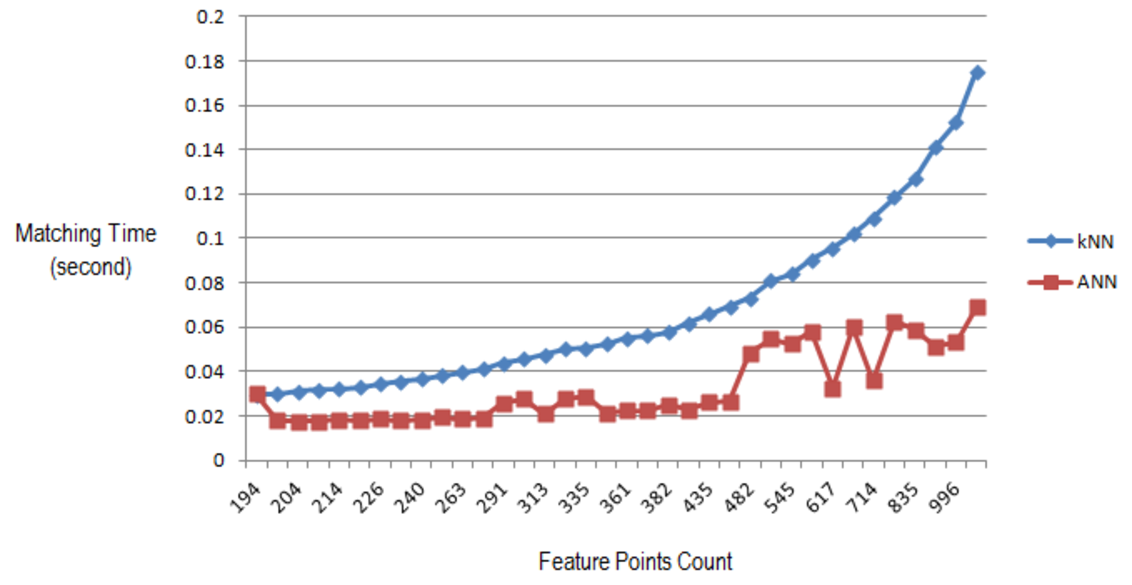
\includegraphics[width=1.2\columnwidth]{2.mainmatter/2.Methodology/figures/SIFT-SURF}%
\caption[Comparison of SIFT and SURF]{Comparison of SIFT and SURF: Feature points versus computational time}%
\label{fig:chart:SIFT-SURF}%
\end{figure}

\noindent SIFT is more accurate because of its high dimensional features, its high computational time is the main drawback making it inappropriate for real time or user-centered applications like medical software. I have chosen SURF method because it is faster and still it gives accurate matches. 

\subsection{kNN versus ANN}
\label{sec:kNN-ANN}
In this section, I will present experimental results on kNN and ANN matching methods for SURF features (64 dimensions) which is presented in graph shown in figure~\ref{fig:knn-ann}. The graph clearly shows that ANN matching always faster than kNN. kNN matching is showing exponential increase in computational complexity when key-points are increased which implies that kNN becomes expensive for large key-points. In practice, we have larger number of feature points to be matched, so ANN matching is preferred to kNN.

\begin{figure}[H]%
\centering
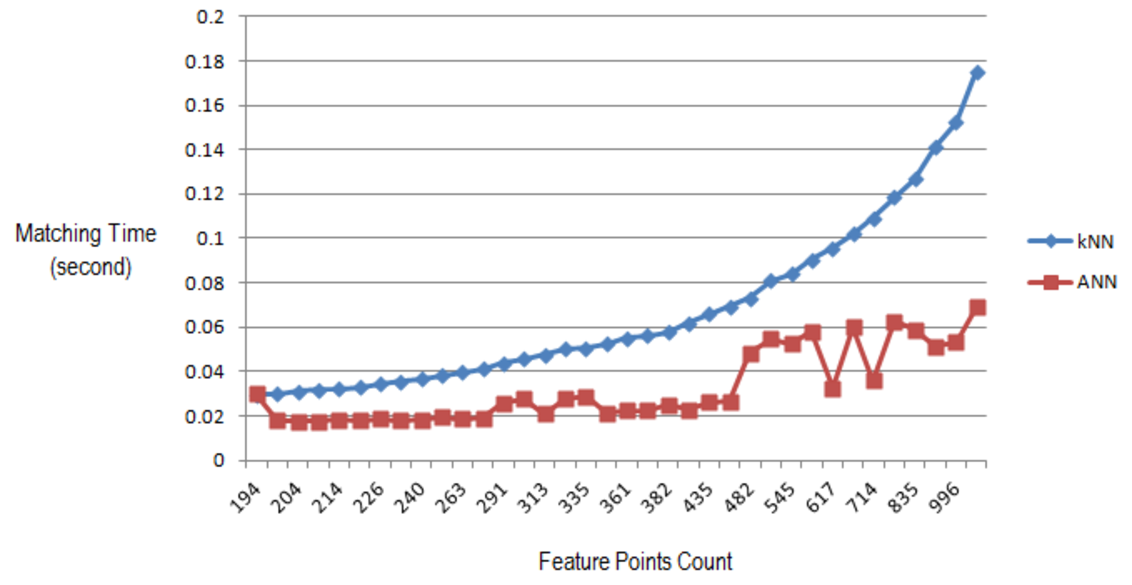
\includegraphics[width=1.3\columnwidth]{2.mainmatter/2.Methodology/figures/kNN-ANN}%
\caption[Comparison of kNN and ANN]{Comparison of kNN and ANN: Feature points vs. matching time}%
\label{fig:knn-ann}% 
\end{figure}

\subsection{Getting Accurate Matches}
\label{sec:accurate-matches}
The nearest neighborhood method just gives the closest point as the matching point which is not necessarily the true match. So, we have to implement tests to remove the false matches identified by nearest neighborhood method. In this section, I implemented some tests to increase the accurate matches by identifying possible false matches. The increment of accurate matches helps to get more accurate transformation model (i.e. \emph{homography}).\\ 

\noindent I have implemented \emph{Ratio} (section~\ref{sec:ratio-test}) and \emph{Symmetry} (section~\ref{sec:symmetry-test}) tests and presented the results in graphical form as shown in figure~\ref{fig:accurate-matches}. The ANN matching resulted 1295 matches (figure~\ref{fig:matches-nn}) , then a significant number of inaccurate matches (1118 matches) are removed by Ratio test (figure~\ref{fig:ratio-test}). For remaining 177 matches, I carried out Symmetry test, which again removed 80 inaccurate matches to get 97 best matches as shown in figure~\ref{fig:symmetry-test}. Although these tests removed significant number of inaccurate matches, the obtained best matches are not 100\% accurate which we can be clearly seen in figure~\ref{fig:symmetry-test}. The remaining inaccurate matches can be identified as outliers by robust estimation methods discussed in the next chapter.


\begin{figure}[H]%
\begin{center}
\subfloat[Nearest neighborhood matches]{\label{fig:matches-nn} 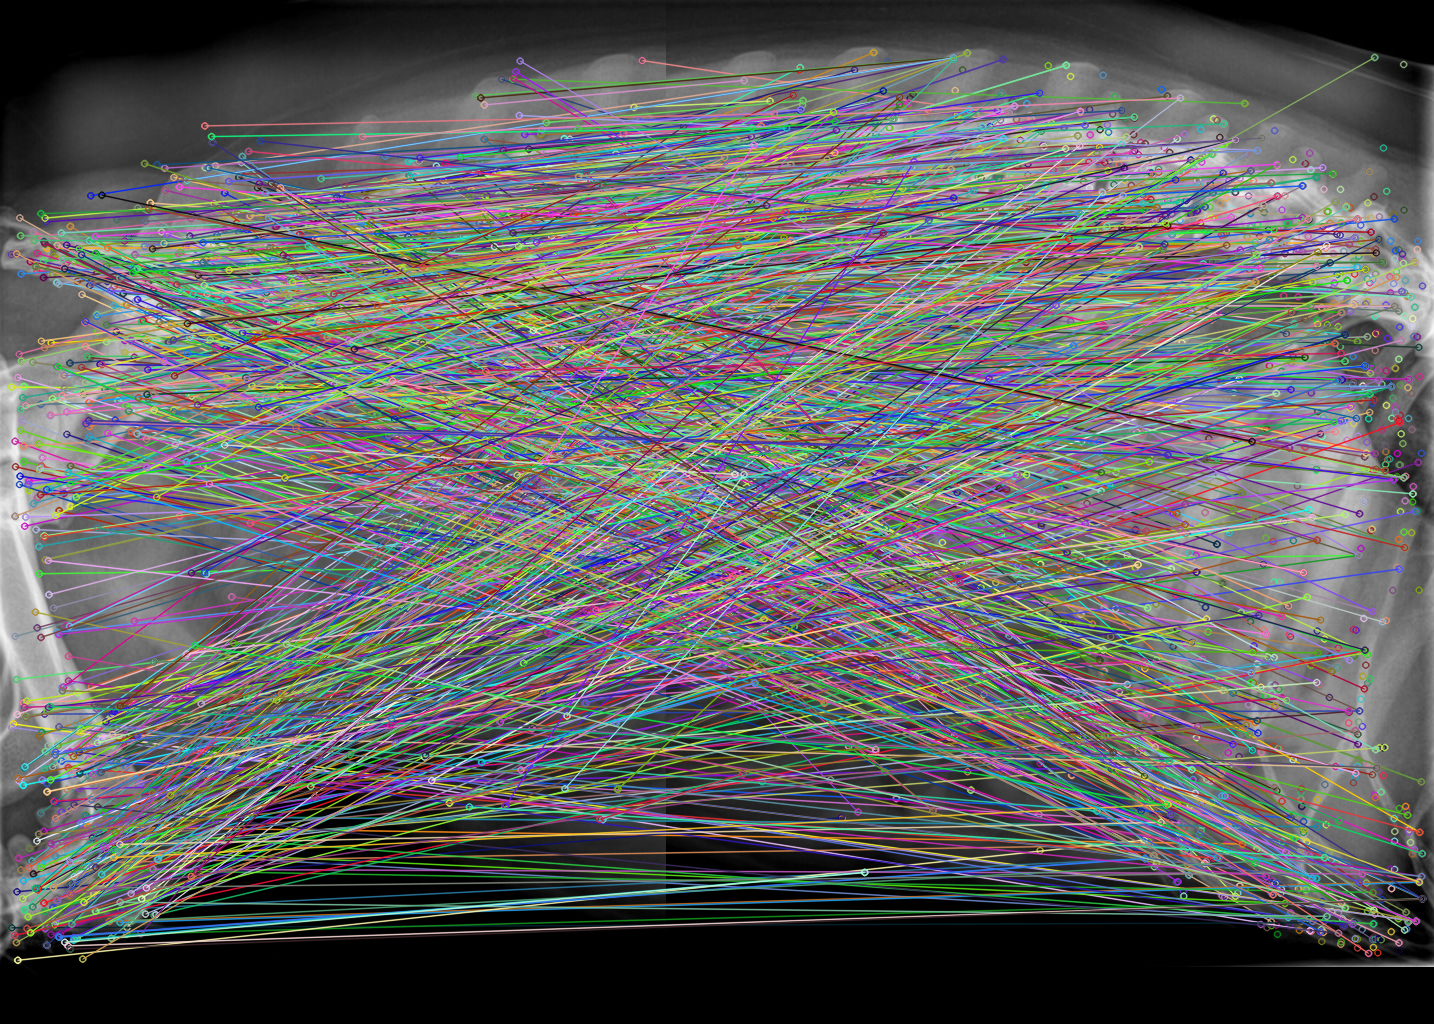
\includegraphics[width= 0.70\columnwidth]{2.mainmatter/2.Methodology/figures/matches}} \hspace{1mm}
\subfloat[Ratio Test] {\label{fig:ratio-test} 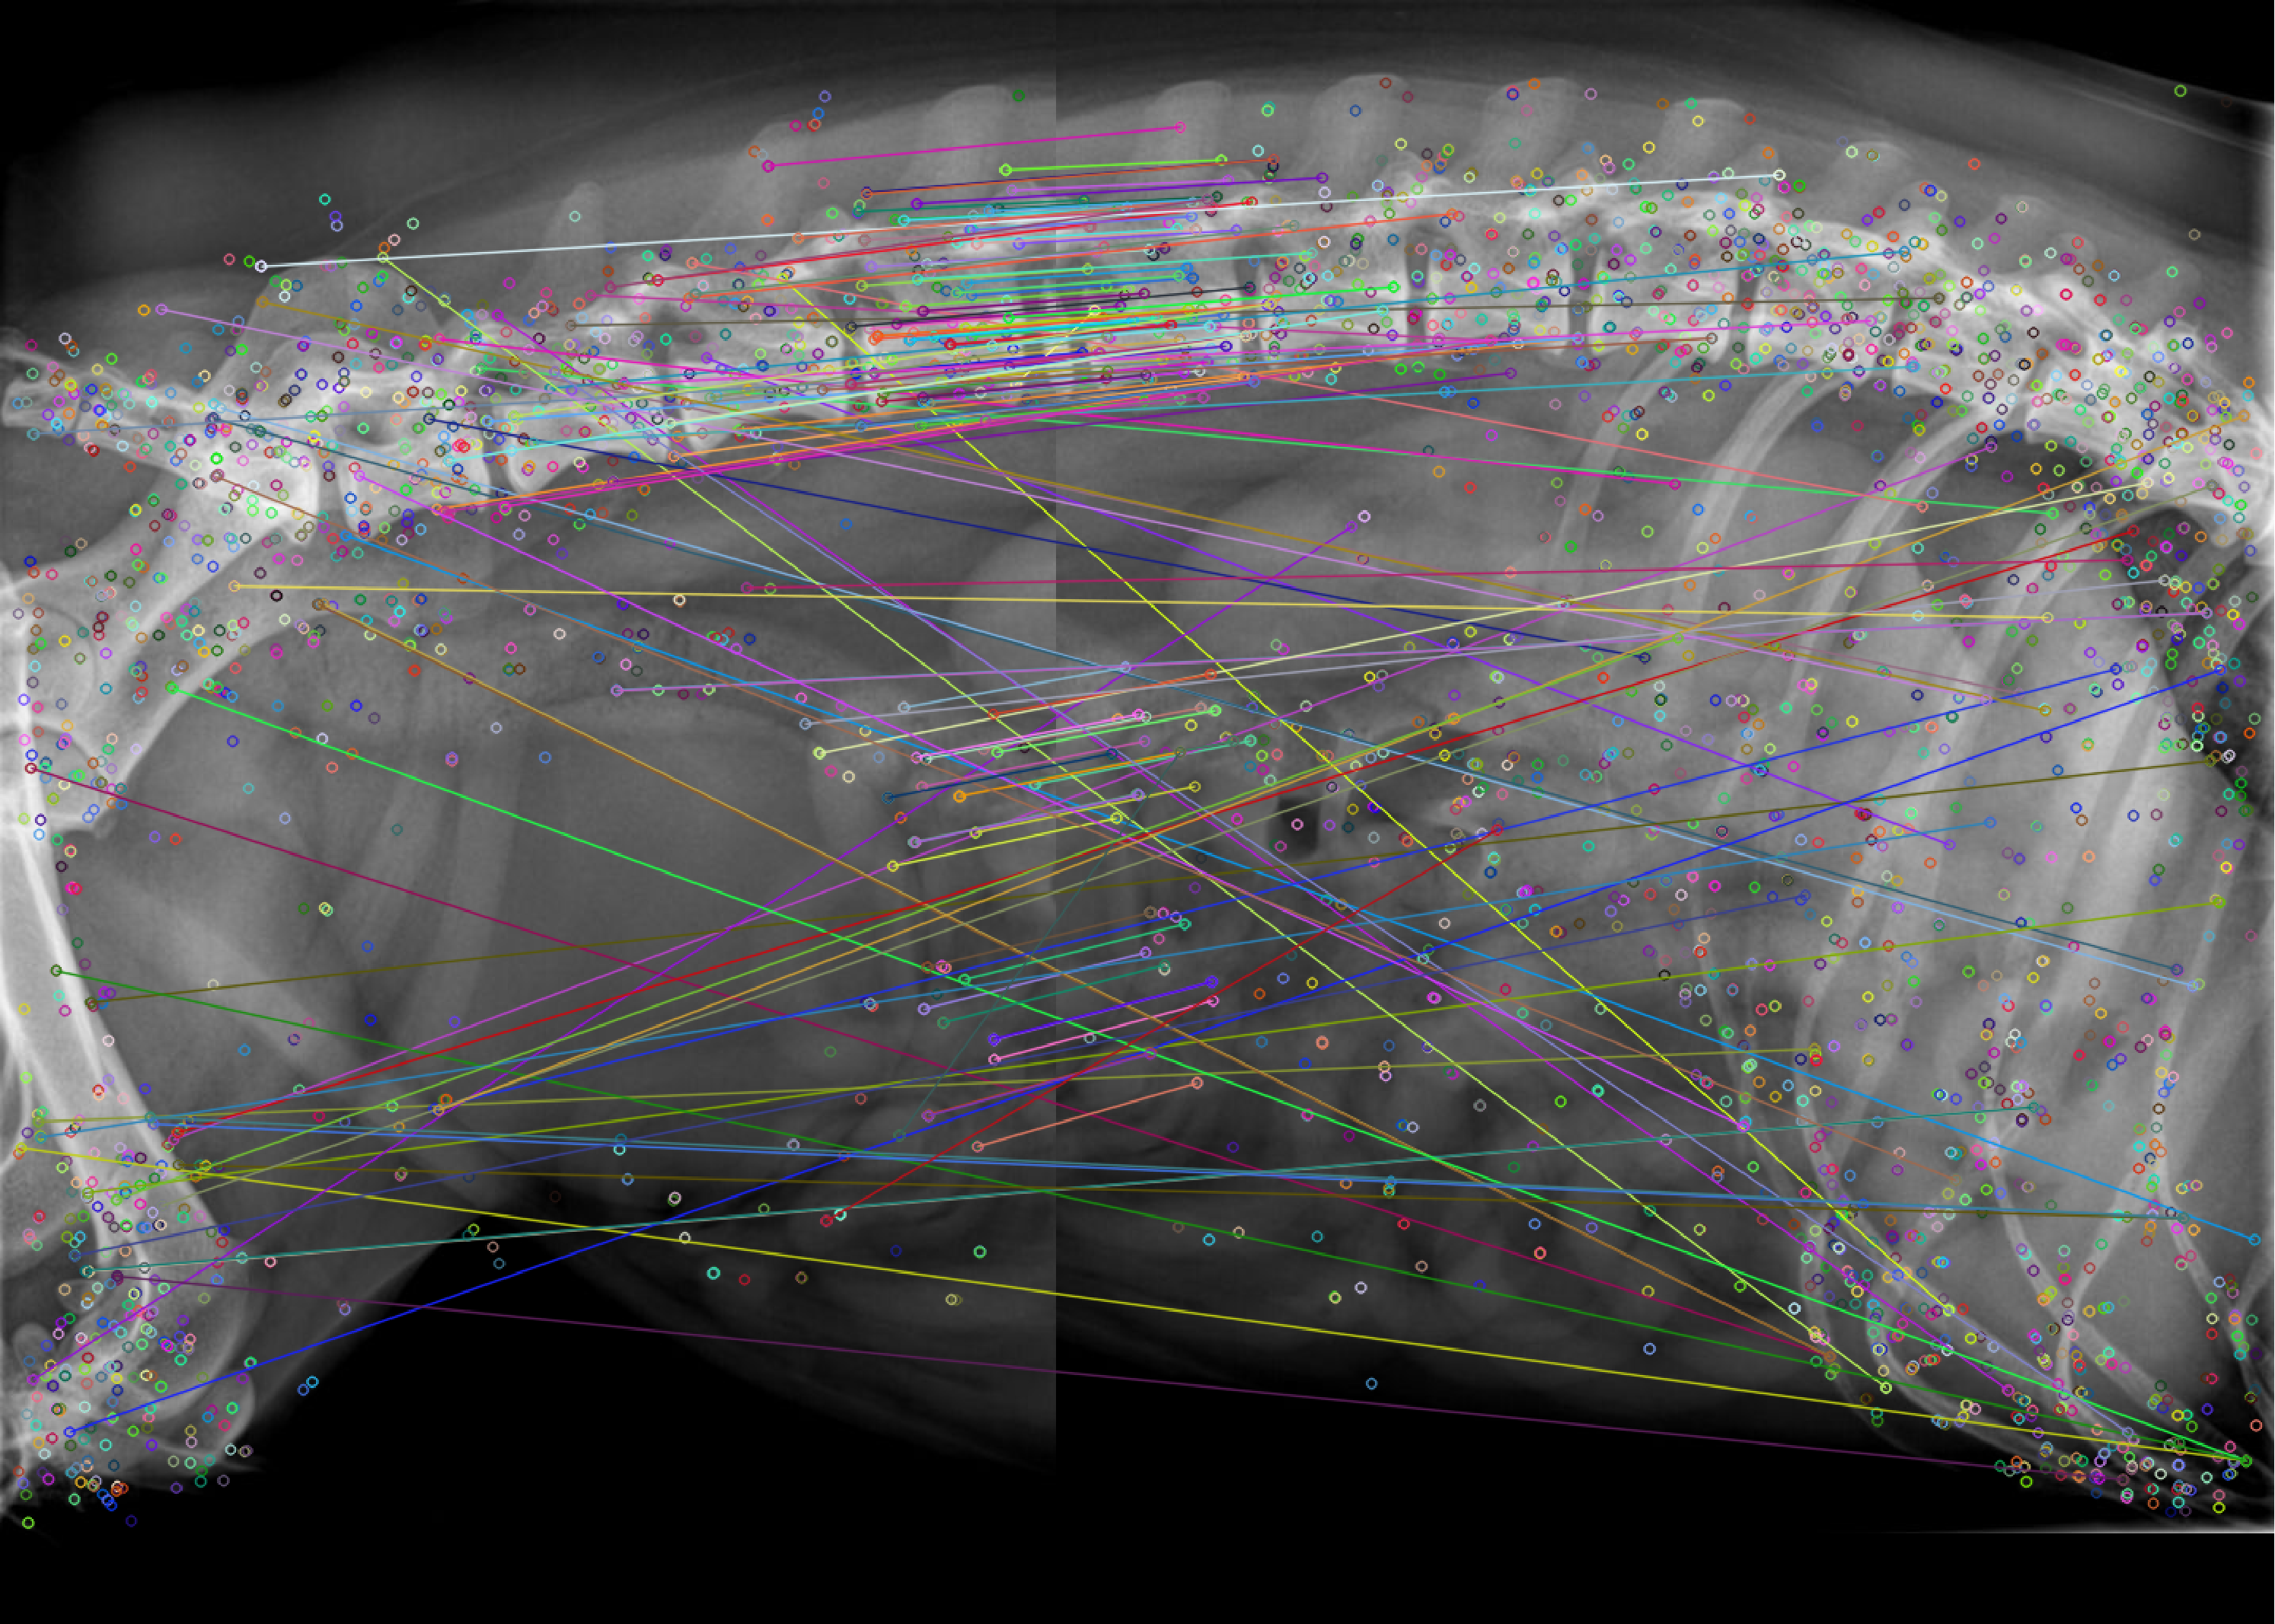
\includegraphics[width= 0.70\columnwidth]{2.mainmatter/2.Methodology/figures/ratio-test}}\quad
\subfloat[Symmetry Test] {\label{fig:symmetry-test} 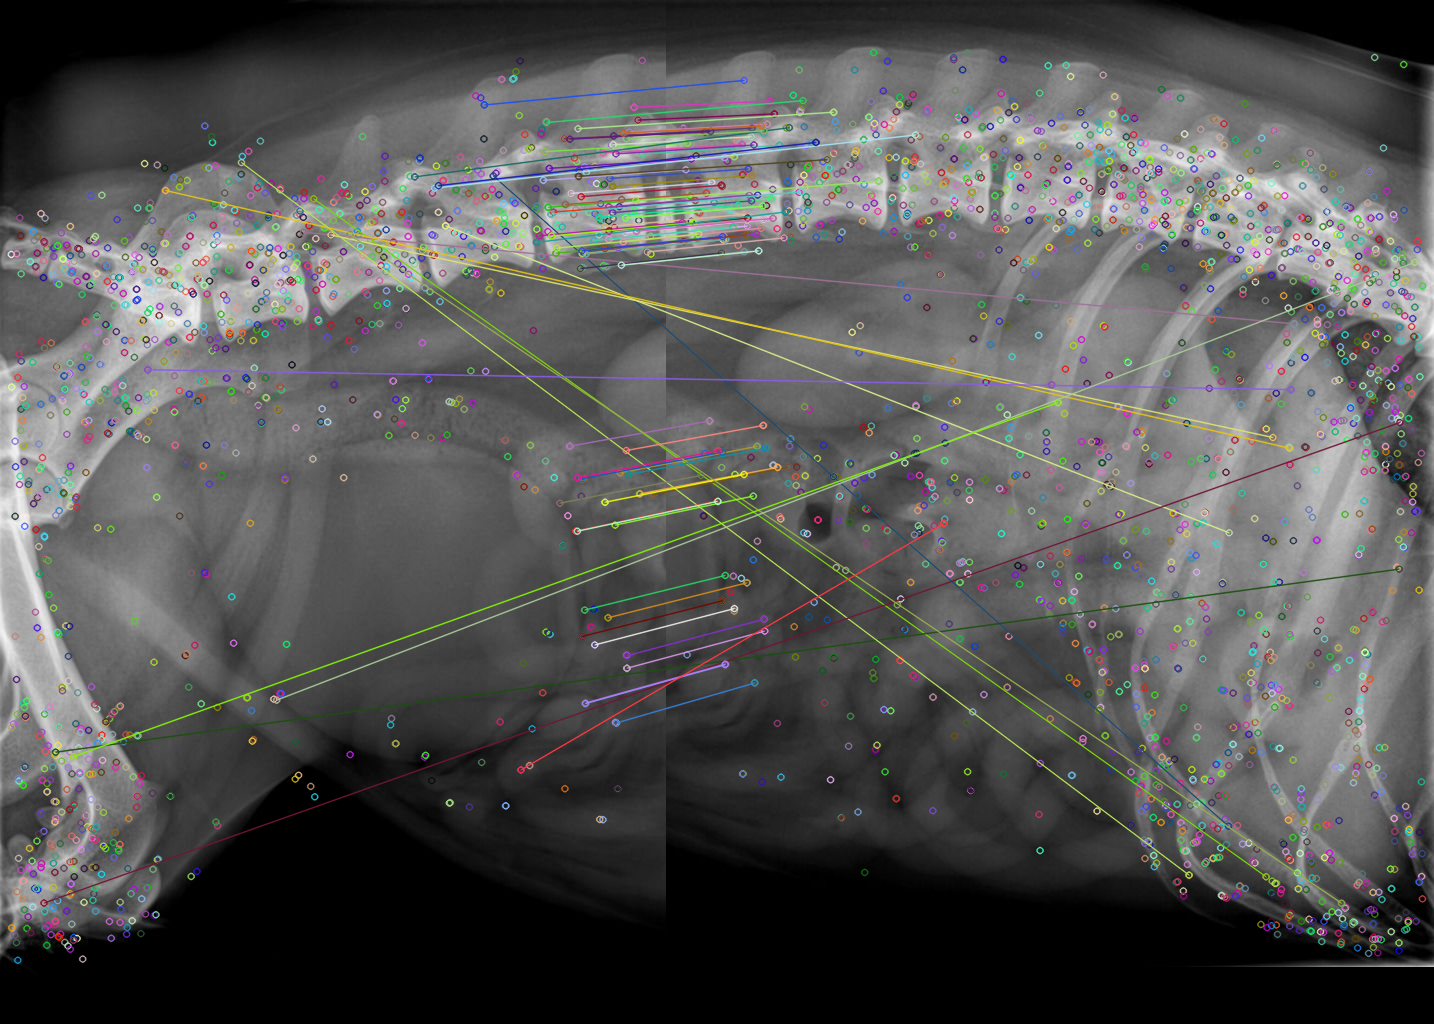
\includegraphics[width= 0.70\columnwidth]{2.mainmatter/2.Methodology/figures/symmetry-test}}
\caption[Steps of Getting Best Matches]{Steps of getting best matches:~\subref{fig:matches-nn} a lot of matches found using NN method~\subref{fig:ratio-test} Ratio test removed a significant number of false matches.~\subref{fig:symmetry-test} The false matches from ratio test are further removed by symmetry test.}%
\label{fig:accurate-matches}%
\end{center}
\end{figure}
